\subsection{ATLAS detector}

The ATLAS detector~\cite{PERF-2007-01, GENR-2019-02} is a general-purpose particle physics detector with symmetrical cylindrical geometry and nearly 4$\pi$ solid angle coverage.\footnote{\AtlasCoordFootnote}
The detector components include inner tracking detectors encased in a superconducting solenoid, electromagnetic (EM) and hadronic calorimeters, and a muon spectrometer which includes three large superconducting toroid magnets.

\subsubsection{Inner Detector}
The inner detector (ID) system tracks charged particles within the range $|\eta|<2.5$ and full coverage in azimuth.
The ID lies inside of a 2 T axial magnetic field, which bends the charged particles so their momentum can be measured.
Counting outward from the beampipe, the first component is the Insertable B-Layer (IBL), which was a new silicon tracker for Run 2 and enhanced tracking performance in high-luminosity data-taking.
The IBL needed to be radiation hard given its close proximity to the beam pipe.
The Pixel detector is next, which is another silicon pixel tracker.
The IBL and Pixel typically provide 4 tracking points for charged particles.
The SemiConductor Tracker (SCT) is a larger, further out tracker that typically provides 8 tracking points.
Finally, the last layer of the ID is the Transition Radiation Detector (TRT), which uses straw drift tubes filled with a Xe-based gas mixture.
The TRT provides basic PID as it is able to discriminate between electrons and photons.
All together, The ID provided precise tracking of charged particles with \PT\ > 0.5 \GeV\
Figure~\ref{fig:atlas_inner_detector} displays the location and appearance of the different ID layers in ATLAS.
\begin{figure}[htbp]
    \centering
    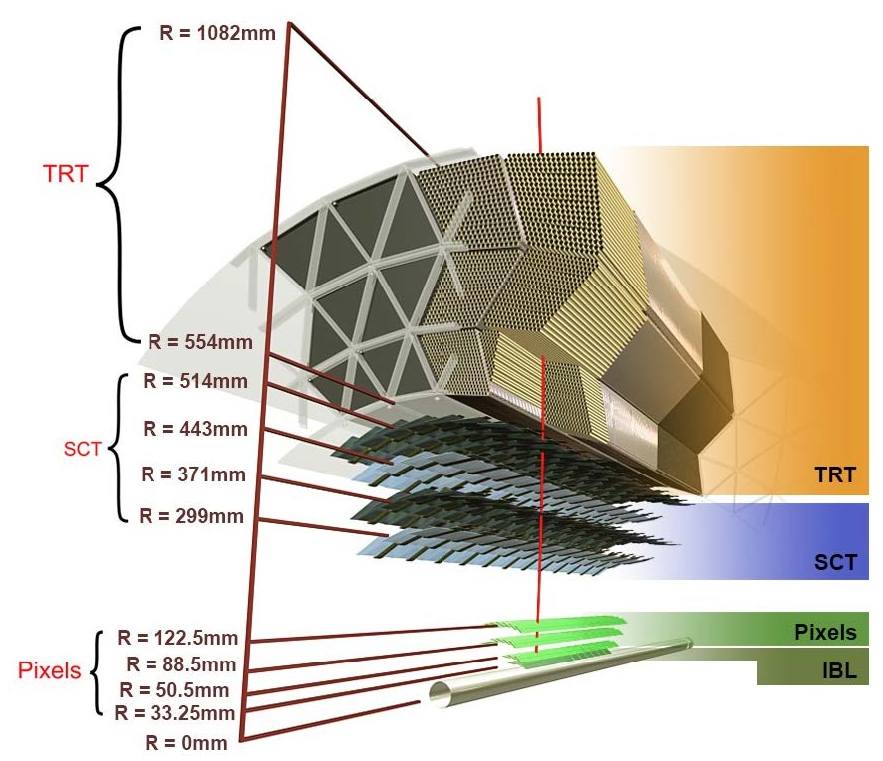
\includegraphics[
        width=0.55\linewidth,
        alt={Exploded view of the ATLAS Inner Detector showing the Insertable B-Layer, pixel detector, semiconductor tracker, and transition radiation tracker, with their radial positions.}
    ]{chapters/the_lhc_and_atlas/figures/atlas_detector/innerdet.png}
    \caption{Schematic layout of the ATLAS Inner Detector, showing the pixel detector, semiconductor tracker (SCT), and transition radiation tracker (TRT). Figure 17 from Reference~\cite{GENR-2019-02}.}
    \label{fig:atlas_inner_detector}
\end{figure}

\FloatBarrier
\subsubsection{Calorimeter System}
The ATLAS calorimeter system consists of two parts, a Liquid Argon (LAr) calorimeter and a scintilating tile calorimeter.
The system destructivly samples particles over a wide range of pseudorapidity (|$\eta$|<4.9) with full coverage in azimuth.
The sampling calorimeter design consists of insterspered absorber material, which cause the incident particles to shower, and active material, which output a signal proportinal to the energy deposited by a secondary particle shower crossing that layer.
Calorimeters typically consist of a EM and then a hadronic calorimeters, where the EM calorimeters are stationed before the hadronic calorimeters.
This setup is because electrons and photons will lose energy over realitvly short distances due to pair production and bremsstrahlung while hadrons take longer distances to shower.
The LAr calorimeter consists of an EM calorimeter, a hadronic end-cap calorimeter (HEC), and a Forward Calorimeter (FCal).
All the parts of the LAr calorimeter use liquid argon as the active material.
The EM calorimeter uses Pb plates as passive material.
Copper was used for the HEC and copper+tungstan were used for the FCal.
Since the HEC and FCal are more geometrically constrained, copper helps with heat dissipation.
The tile calorimeter sits outside of the LAr calorimeter in the central $\eta$ region; it uses steel tiles as an absorber and scintilating tiles as the active material.
A diagram of the calorimeter system, with the different subcompoenets highlighted can be seen in Figure~\ref{fig:atlas_calorimeter_cross_section}.
Different $\eta$ coverages are denoted on the plot.

\begin{figure}[htbp]
    \centering
    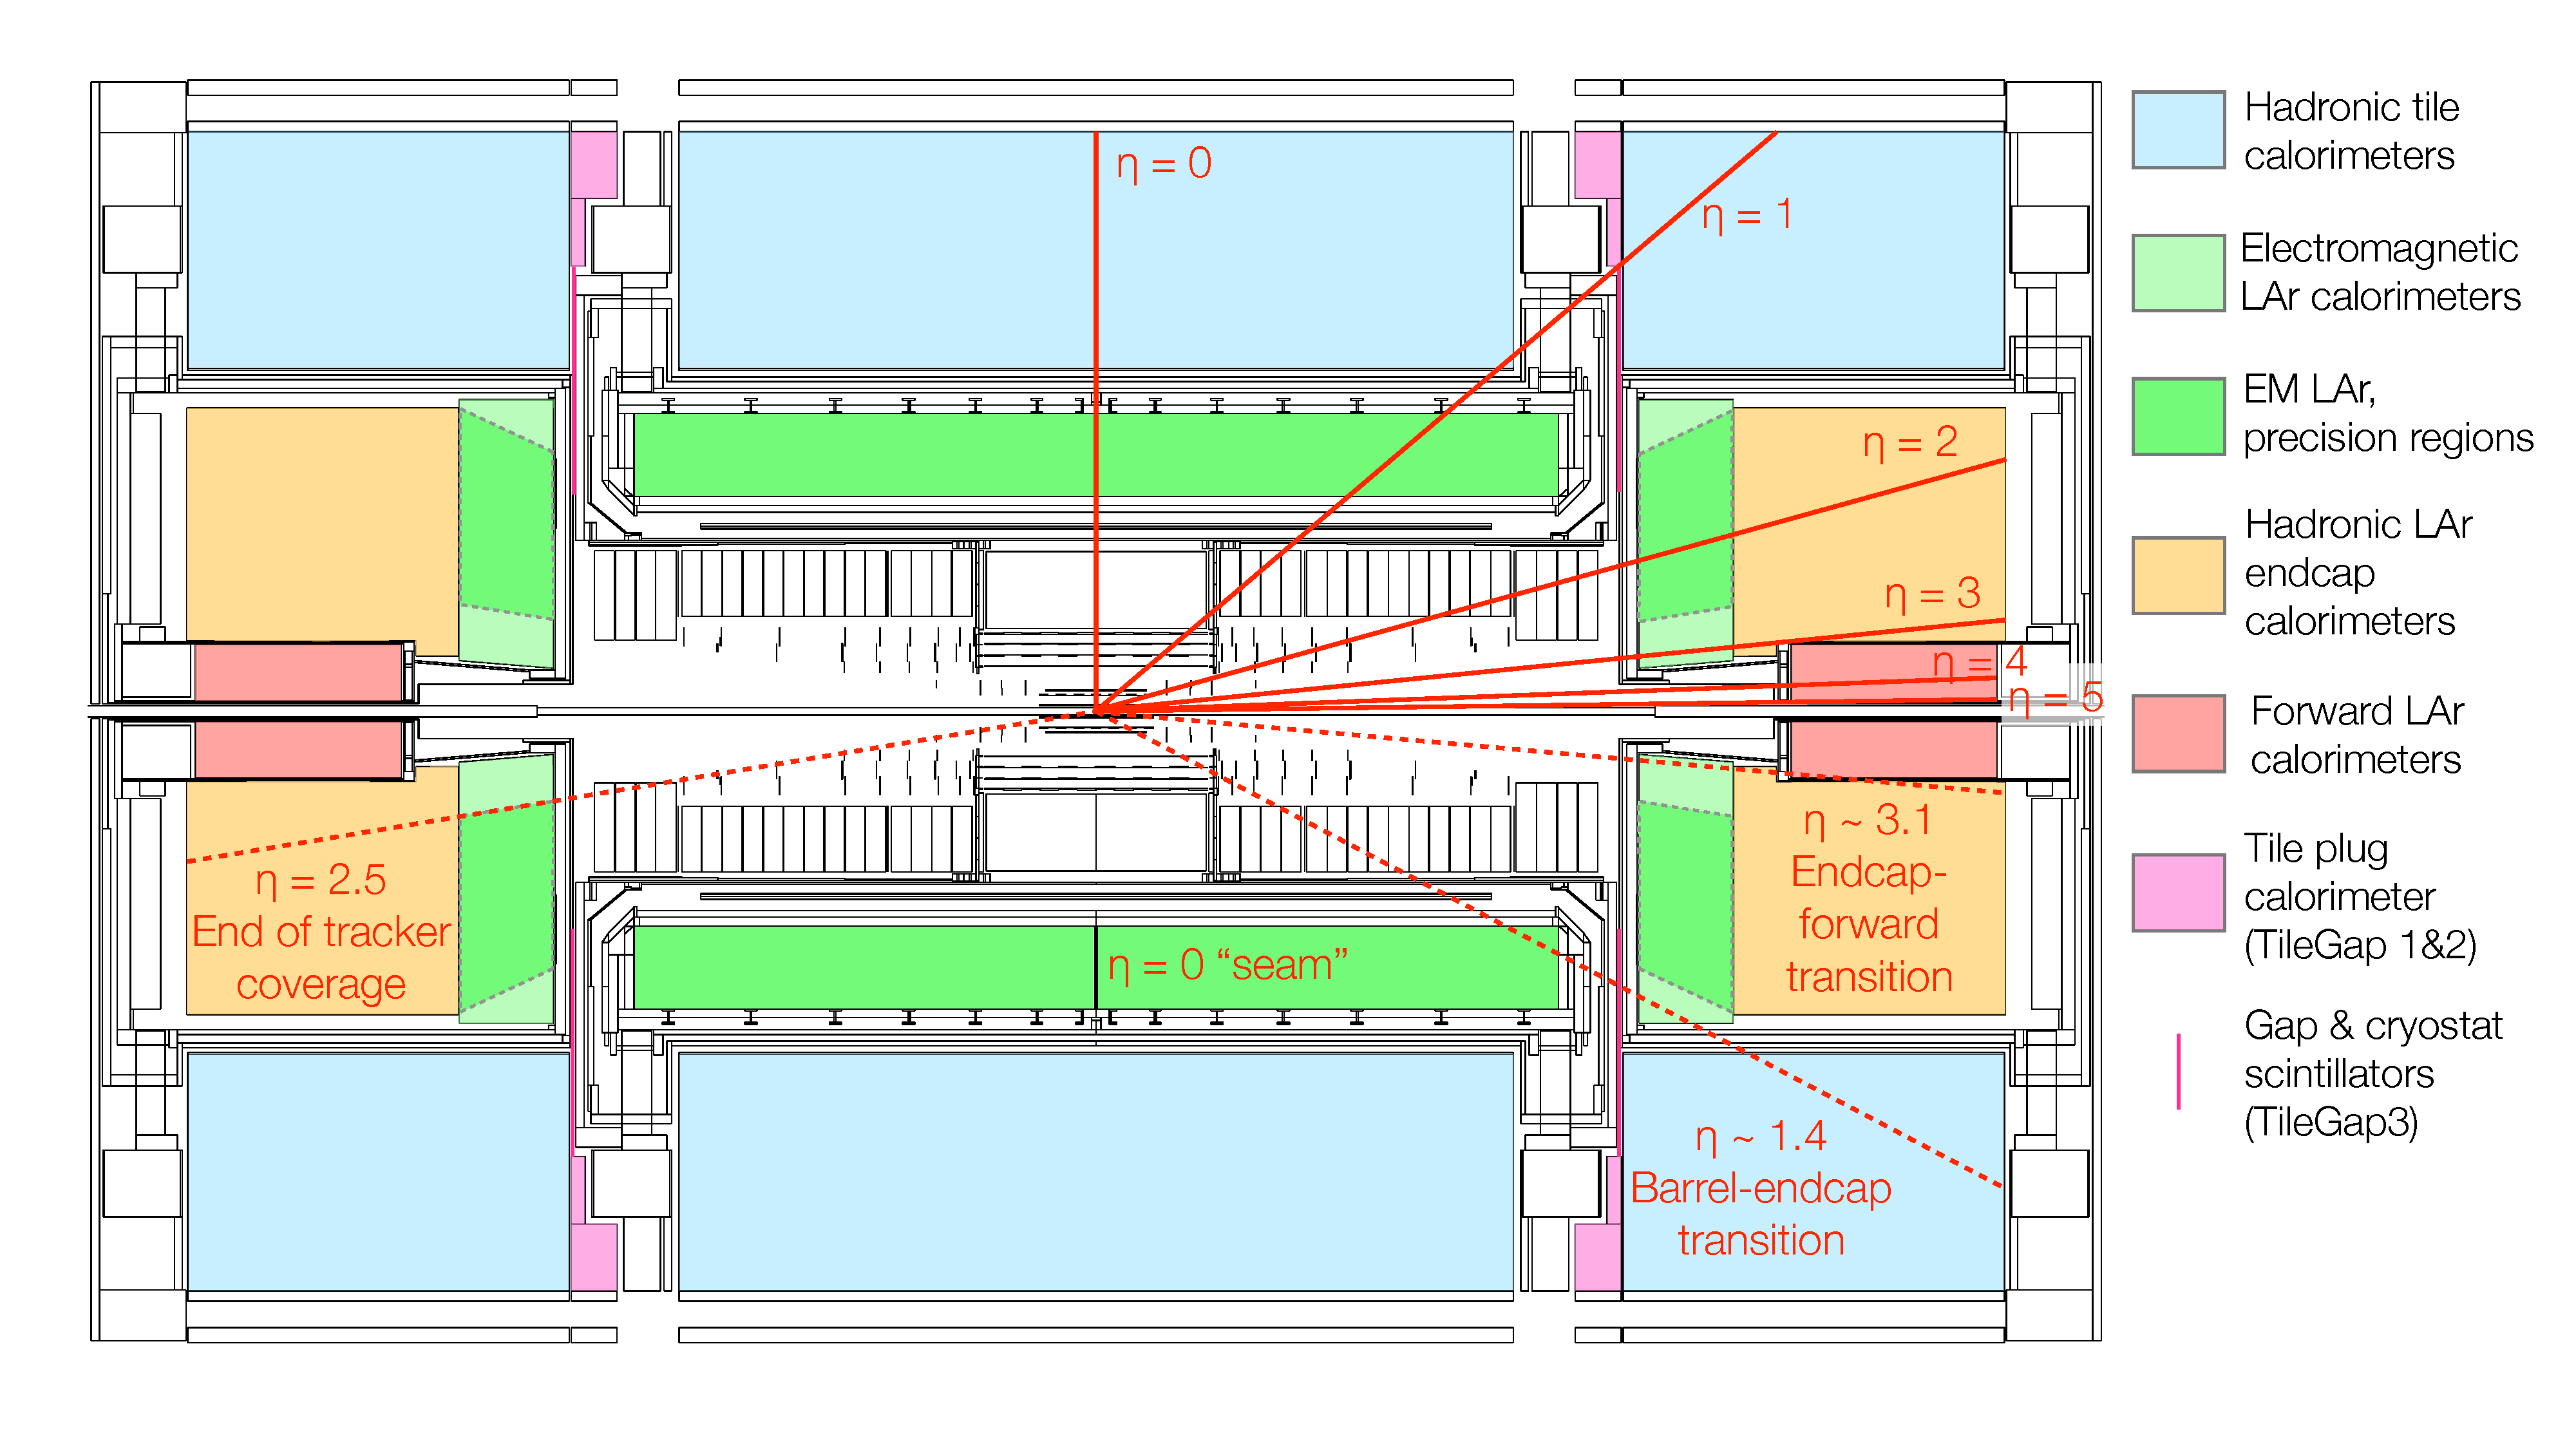
\includegraphics[
        width=0.8\linewidth,
        alt={Cross-sectional diagram of the ATLAS calorimeter system, showing its electromagnetic and hadronic calorimeter components.}
    ]{chapters/the_lhc_and_atlas/figures/atlas_detector/atlascalocrosssection.pdf}
    \caption{Cross section of the ATLAS calorimeter system. Figure 1 from Reference~\cite{JETM-2018-05}.}
    \label{fig:atlas_calorimeter_cross_section}
\end{figure}

The material budget for the ATLAS calorimeter is displayed in the left panel of Figure~\ref{fig:atlas_calorimeter_material_pulse}, measured in units of nuclear interaction length.
Over all pseudorapidity particles must traverse at least 9 nuclear interaction lenghts, ensuring that at least 99.98\% of hadronic energy is deposited in the calorimeter.

\begin{figure}[htbp]
    \centering
    \begin{subfigure}[t]{0.49\linewidth}
        \centering
        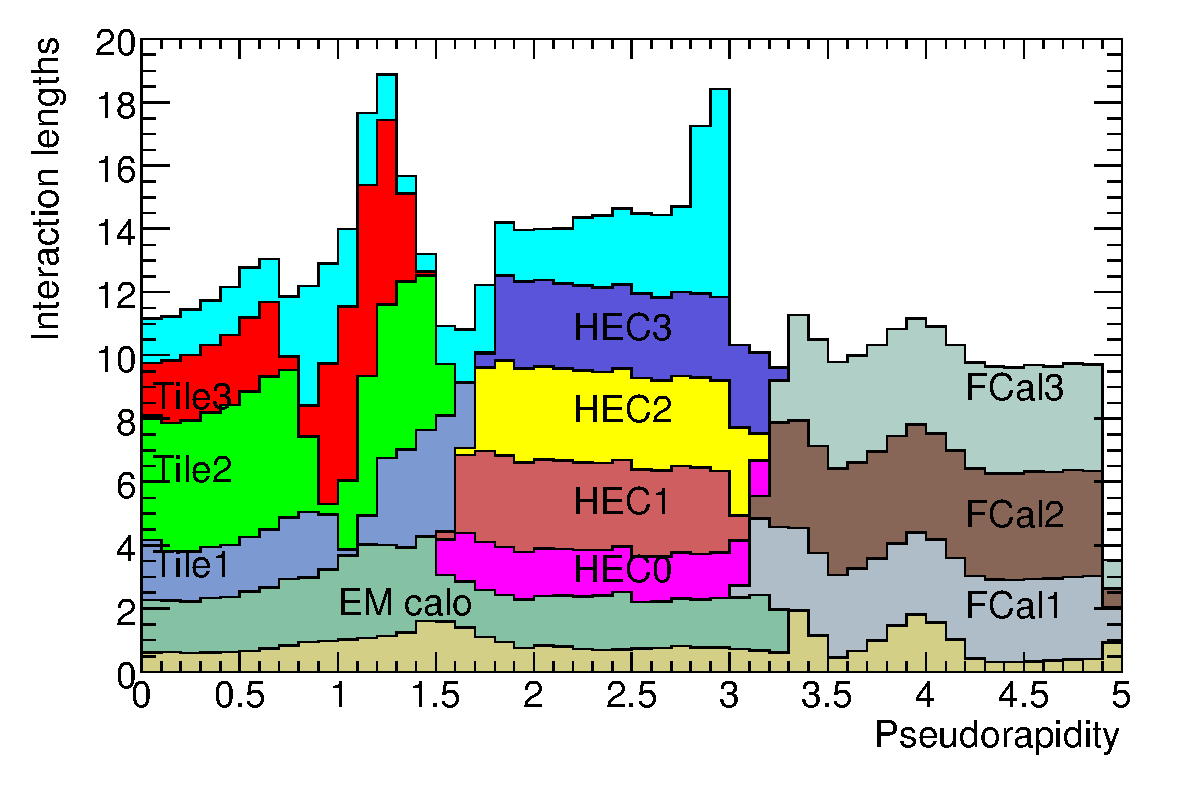
\includegraphics[
            width=\linewidth,
            alt={ATLAS calorimeter material budget as a function of pseudorapidity, showing contributions from detector materials.}
        ]{chapters/the_lhc_and_atlas/figures/atlas_detector/calomaterialbudget.pdf}
    \end{subfigure}
    \hfill
    \begin{subfigure}[t]{0.36\linewidth}
        \centering
        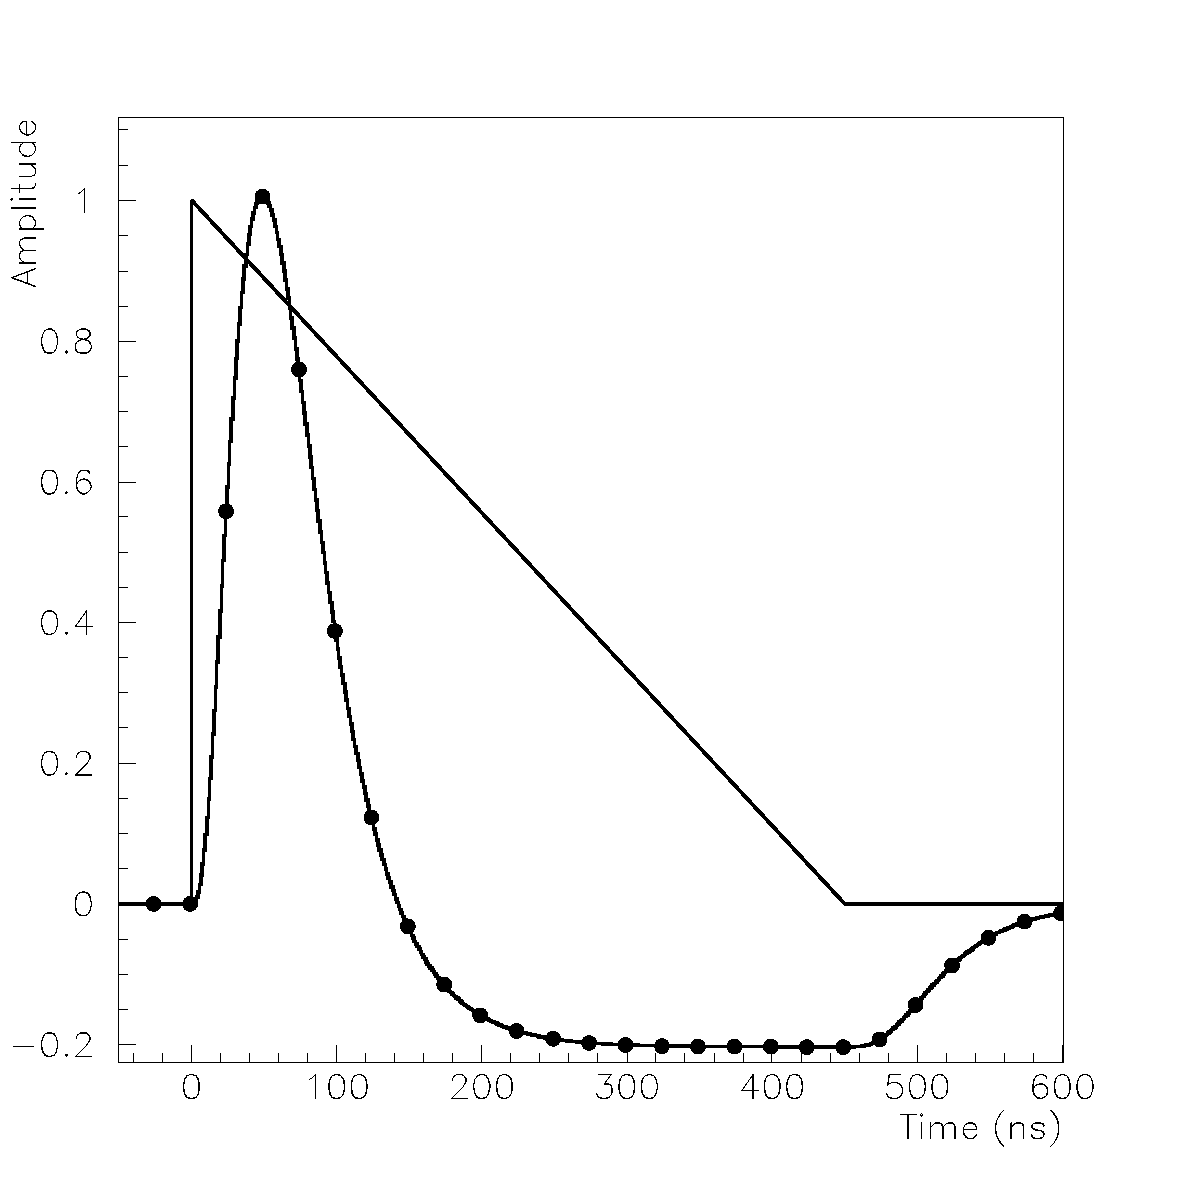
\includegraphics[
            width=\linewidth,
            alt={Liquid-argon calorimeter pulse shape showing the bipolar signal and its undershoot.}
        ]{chapters/the_lhc_and_atlas/figures/atlas_detector/larOvershootPulse.pdf}
    \end{subfigure}
    \caption{ATLAS calorimeter properties. Left: Material budget as a function of pseudorapidity (Figure 75 from Reference~\cite{PERF-2007-01}). Right: Liquid-argon calorimeter pulse shape and undershoot (Figure 103 from Reference~\cite{PERF-2007-01}).}
    \label{fig:atlas_calorimeter_material_pulse}
\end{figure}
In ATLAS, transverse energy (\ET\ ) deposited in the FCal is the most common type of centrality estimator (CE) used for Heavy Ion analyses.
The \ET\ can be shown to be very well corratlted to the charged particle multiplicity at midrapidity.
This \ET\ is calibrated to the EM scale, so the absolute energy scale is not gaurenteed to be correct when hadrons impinge on the detector.
One problem that can effect centrality determination in this way is the presence of out-of-time pileup.
The right panel of Figure~\ref{fig:atlas_calorimeter_material_pulse} shows an example of a pulse shape in the LAr calorimeter.
One can see that after a large pulse, the LAr readout amplitude will go negative for a long time (around 25 BCIDs).
For heavy ion collisions, this can mean that an event that is preceeded by another high-activity event can have its energy measure biased.
This is one of the reasons out-of-time pileup must be rejected in analyses utilizing centrality.

\FloatBarrier
\subsubsection{Muon Spectrometer}
Muons weakly interact with ordinary matter and as such are able to escape the ID and calorimeter systems while losing little energy.
As such a dedicated spectrometer is built surrounding these systems to identify and track muons over a pseudorapidity range of $|\eta| < 2.7$  with full coverage in azimuth.
The muons are deflected by a set of superconducting air-core toroidal magnets with a strength of 2.0--6.0 T$\cdot$m.
The spectrometer is built out of three layers, each made up of monitored drift tubes.
To provide additional tracking precision, cathode-strip chambers were implemented in the endcap region in Run~2, but these were replaced by ``so-called'' the New Small Wheel detectors, which are small-strip thin-gap chambers and Micromegs champers in Run~3.
The muon trigger covers a slightly smaller range of pseudorapidity of $|\eta| < 2.4$.

\FloatBarrier
\subsubsection{Forward Detectors}
The ATLAS forward detectors lie along the beampipe and cover very forward ranges of rapidity detecting particles that are missed by the coverage of the ATLAS central detector.

\paragraph{LUCID}

\paragraph{AFP}

\paragraph{ALFA}

\paragraph{ZDC} The Zero Degree Calorimeter (ZDC) is a detecrtor employed mostly for heavy ion specific runs in the LHC.
The author of this dissertation is a member of the ZDC group and as such this detector deserves a more detailed discussion, which is be given in Section~\ref{sec:ZDC}

\FloatBarrier
\subsubsection{Trigger and Software}

The author of this dissertation is a member of the ATLAS collaboration, and the ATLAS detector was used for all measurements described.
